%standard 2.3

%start_of_questions


%new_question
%%%%%%%%%%%%%%%%%%%%%
	% Problem 5
	% Difficulty: 3
%%%%%%%%%%%%%%%%%%%%%
	\item
		Write a program that calculates the volume of a cylinder.  The user should be able to pick
		the height and radius.  Use the value of $\pi$ from the math module in your calculation.\\
		\tab Hint: $V = \pi r^2 h$\\

		\vspace*{-2em}
		\begin{flushright}
		\begin{tikzpicture}
			\node (a) [cylinder, shape border rotate=90, draw, 
				minimum height=25mm, minimum width=15mm] {};
			\draw [<->] ([xshift=5pt]a.before bottom) -- ([xshift=5pt]a.after top)
				 node [midway, right] {$h$};
			\draw [->] ([yshift=-5pt]a.bottom) -- ([yshift=-5pt]a.bottom -| a.before bottom)
				node [midway, below] {$r$};
		\end{tikzpicture}
		\end{flushright}


%new_question
%%%%%%%%%%%%%%%%%%%%%
	% Problem 6
	% Difficulty: 3
%%%%%%%%%%%%%%%%%%%%%
	\item
		Write a program that calculates and then outputs the volume of a sphere.  
		The user should be able to pick the radius.
		Use the value of $\pi$ from the math module in your calculation.\\	
		Hint: $V = \dfrac{4}{3}\pi r^3 $
	
		\begin{flushright}
			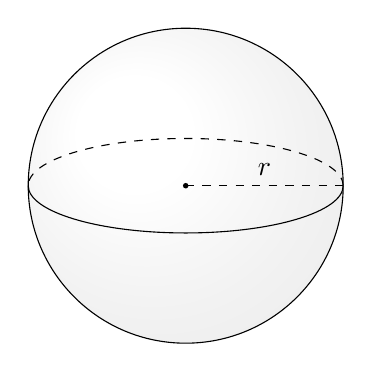
\begin{tikzpicture}
			\shade[ball color = white, opacity = 0.1] (0,0) circle (2cm);
			\draw (0,0) circle (2cm);
			\draw (-2,0) arc (180:360:2 and 0.6);
			\draw[dashed] (2,0) arc (0:180:2 and 0.6);
			\fill[fill=black] (0,0) circle (1pt);
			\draw[dashed] (0,0 ) -- node[above]{$r$} (2,0);
			\end{tikzpicture}
		\end{flushright}





%new_question
%%%%%%%%%%%%%%%%%%%%%
	% Problem 7
	% Difficulty: 3
%%%%%%%%%%%%%%%%%%%%%
	\item 
		Write a program that calculates then outputs the volume of a cone.  \\
		The user should be able to pick $r$ (the radius) and $h$ (the height).\\
		Use the value of $\pi$ from the math module in your calculation.\\	
		Hint: $V = \pi \cdot \dfrac{r^2 h}{3}$ \vspace*{-5em}
		\begin{flushright}
		\begin{tikzpicture}
			\draw[dashed] (0,0) arc (170:10:2cm and 0.4cm)coordinate[pos=0] (a);
			\draw (0,0) arc (-170:-10:2cm and 0.4cm)coordinate (b);
			\draw[densely dashed] ([yshift=4cm]$(a)!0.5!(b)$) 
				-- node[right,font=\footnotesize]{$h$}coordinate[pos=0.95] (aa)($(a)!0.5!(b)$)
				-- node[below,font=\footnotesize] {$r$}coordinate[pos=0.1] (bb) (b);
    		\draw (aa) -| (bb);
    		\draw (a) -- ([yshift=4cm]$(a)!0.5!(b)$) -- (b);
  		\end{tikzpicture}
	\end{flushright}





%new_question
%%%%%%%%%%%%%%%%%%%%%
	% Problem 8
	% Difficulty: 3
%%%%%%%%%%%%%%%%%%%%%
	\item
		Write a program that calculates and then outputs the area of a semi--circle.  	
		The user should be able to pick the radius.
		Use the value of $\pi$ from the math module in your calculation.\\	
		Hint: $A = \dfrac{1}{2}\pi r^2 $
	
		\begin{flushright}
			\begin{tikzpicture}[baseline=(current bounding box.north)]
				\begin{scope}
		    		\clip (-1.5,0) rectangle (1.5,1.5);
		    		\draw (0,0) circle(1.5);
					\draw (-1.5,0) -- (1.5,0);
					\draw[dashed] (0,0) -- (0,2);
				\end{scope}
				\node[below right= 1mm of {(0,1)}] {$r$};
			\end{tikzpicture}
		\end{flushright}

%end_of_questions

